\chapter{Felhasználói dokumentáció} % User guide
\label{ch:user}

Ezen fejezet a felhasználó részletes tájékoztatására szolgál. Az alfejezetek az alkalmazás szükséges előfeltételeit, telepítési és használati információkat tartalmaznak. A program technikai részletekbe menő dokumentációját a \ref{ch:impl} . fejezet (Fejlesztői dokumentáció) tartalmazza.


\section{Röviden az agilis módszertanról és a  "scrum"-ról} % Briefly about the "scrum" 

\begin{description}
	\item[Mi az agilis módszertan?] A szoftverfejlesztési módszerek egy csoportja, ahol a követelmények és megoldások szoros együttműködésén keresztül fejlődnek az önszerveződő  és 		     	multifonkcionális csapatok. Ez elősegíti az korai szállítást, folytonos továbbfejlesztést és bátorít a változásokra adható gyors és rugalmas válaszokra. \footnote{Részletes leírás 		 	   	megtalálható: \url{https://www.agilealliance.org/agile101/}}
	\item[Mi a "scrum"?] Az agilis módszertanon belül sokféle irányzat van, ezek egyike a scrum. A scrum középpontjában a kis létszámú, önszerveződő agilis csapatok állnak. Itt,
 szemben a többi agilis ágazattal, nincsenek általánosan megszabott ,egész rendszert egybefogó szállítási és frissítési időpontok, hanem az aktuális fejlesztések Sprintekbe rendeződnek és ezek lejárta után történik az átadás. Ez közvetlenebb visszajelzést is biztosít a szállító és a kliens között. A scrum szerkezeti felépítése a következő: van egy scrum master, aki egybe fogja a csapat működését, feldata a scrum "menedzselése" gyakorlatilag. Mellete a csapat tartalmaz természetesen fejlesztőket és tesztelőket. A scrum létszáma nincsen hivatalosan meghatározva, de ajánlatos 8-10 főnél nem nagyobbra nőnie, ugyanis így veszít hatékonyságából. A csapatok minden nap egy meghatározott időpontban tartanak stand up-okat, amelyeken minden tag beszámol feladatairól, haldásáról, így mindenki a csapaton belül képbe kerülhet a Sprint aktuális állásáról.
\end{description}

Pár fontosabb fogalom, amely a későbbiekben külön fejezetben részletezve lesz:
\begin{itemize}
	\item Projekt \ref{projects}. fejezet
	\item Epic \ref{stories}. fejezet
	\item User stories \ref{stories}. fejezet
	\item Task \ref{stories}. fejezet
	\item Issue \ref{stories}. fejezet
	\item Kanban \ref{Kanban}. fejezet
\end{itemize}

\newpage

\section{Rendszerkövetelmények} % System requirements

\textbf{Minimum követelmények}: A ScumHelper egy webes alkalmazás. Ez azt jelenti, hogy a felhasználónak csak egy böngészőre van szüksége a számítógépén (például: Google Chrome, Mozilla Firefox, Safari, stb.) és természetesn internet elérésre ahhoz, hogy futtatni tudja a szoftvert. Utóbbi elengedhetetlen, ugyanis csak bejelentkezve lehetséges használni, továbbá internet kapcsolat nélkül a számítógép csak a gyorsírótárában mentett oldalakat tudja megnyitni, de módosításokat nem tudunk végrehajtani az oldalon és váltani sem tudunk az alkalmazáson belül. Nincsen megkötés operációs rendszer tekintetében sem, tehát minden, napjainkban használatos rendszeren (Linux, Windows, Mac OS) egyaránt használható.  

\textbf{Ajánlott követelmények}: A jobb felhasználói élmény érdekében érdemes legalább 1280x720 felbontású kijelzőn használni és a korábban már felsorolt, jelenleg leggyorsabbnak és legbiztonságosabbnak számító böngészővel megnyitni : Chrome, Mozilla firefox, Chromium.

\section{Telepítés}

A felhasználói oldalról nem igényel telepítést. Az eléréshez a szerver elérési URL-jére van szükség, illetve egy felhasználó igénylésére az aktuális rendszergazdától. Érdemes az új felhasználóba való belépés után megváltoztatni jelszavunkat biztonsági okokból.

Rendszergazdai oldalról ha még nem rendelkezik felhasználóval, akkor a fejlesztői dokumentációban (\ref{ch:impl}. fejezet) található részletesebb információ az alkalmazás beüzemelésésől, illetve rendszergazdai felhasználó létrehozásának lépéseiről. 

\newpage

\section{Az alkalmazás felépítése}

\subsection{Bejelentkezés, felhasználók}

Az alkalmazásban az első képernyő, amely fogadja a felhasználót az a login oldal. A ScrumHelper-t csak sikeres bejelentkezés után lehetséges használni. Ha nem rendelkezik felhasználóval, akkor keresse meg a rendszergazdát, és igényeljen egyet. Az egyes felhasználói fiókok egy-egy jogosultsági csoporthoz kötöttek. 

A felhasználói csoportok és jogosultságaik:

\begin{table}[H]
	\centering
	\begin{tabular}{ | m{0.25\textwidth} | m{0.65\textwidth} | }
		\hline
		\textbf{Csoport} & \textbf{Jogosultságok} \\
		\hline \hline
		\emph{Fejlesztő} & projekt/epic/story/task/issue létrehozás/szerkeztés, komment létrehozás/törlés, saját munkaidő napló létrehozása/törlése, Dokumentum feltöltés (ha projekt tulajdonos, akkor törlés), jelszóváltás \\
		\hline
		\emph{Tesztelő} &   projekt/epic/story/task/issue létrehozás/szerkeztés, komment létrehozás/törlés, saját munkaidő napló létrehozása/törlése, Dokumentum feltöltés (ha projekt tulajdonos, akkor törlés), jelszóváltás \\
		\hline
		\emph{Scrum master} & projekt/epic/story/task/issue létrehozás/szerkeztés/törlés, komment létrehozás/törlés, saját munkaidő napló létrehozása/törlése/egész scrum könyvelés megjelenítése, Dokumentum feltöltés (ha projekt tulajdonos, akkor törlés), jelszóváltás \\
		\hline
		\emph{Projekt menedzser} & projekt/epic/story/task/issue létrehozás/szerkeztés/törlés, komment létrehozás/törlés, saját munkaidő napló létrehozása/törlése/egész scrum könyvelés megjelenítése, Dokumentum feltöltés (ha projekt tulajdonos, akkor törlés, jelszóváltás) \\
		\hline
		\emph{Rendszergazda} & minden jogosultsággal rednelkezik, létre is hozhat új csoportokat, kezelheti azok jogosultságait, illetve a felhasználókat is tudja szerkezteni/törölni \\
		\hline
	\end{tabular}
	\caption{Jogosultsági csoportok és jogosultságaik}
	\label{tab:example-1}
\end{table}

\subsection{Főoldal}

\begin{figure}[H]
	\centering
	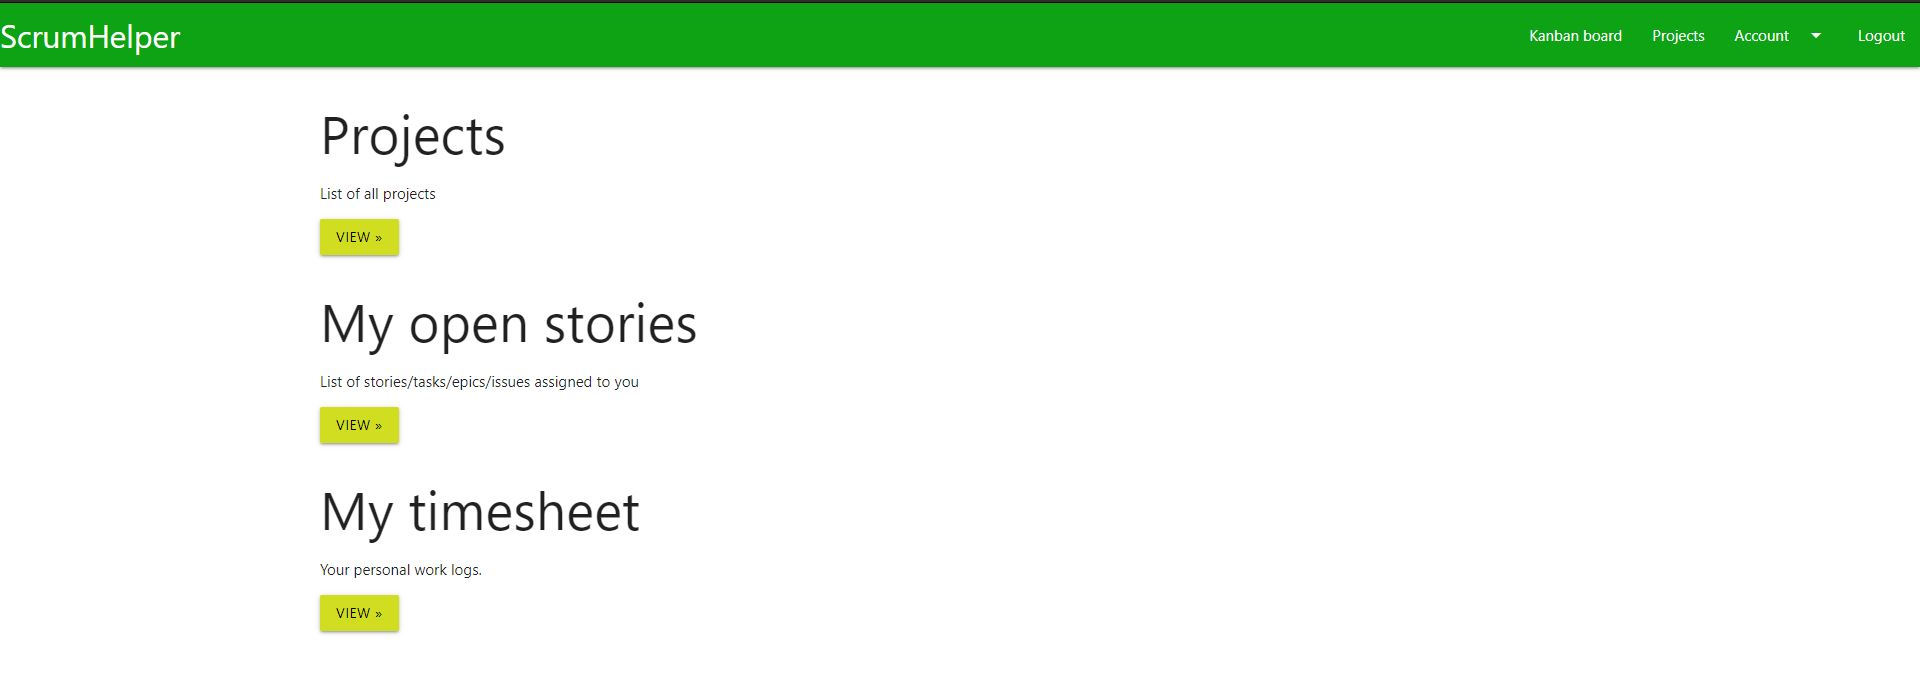
\includegraphics[width=1\textwidth,height=175px,frame]{index_page}
	\caption{Főoldal}
	\label{fig:example-1}
\end{figure}

A \ref{fig:example-1}. ábrán látható a főoldal kinézete. A navigációs sávban az alklamazás neve, Kanban board, Projects, Account és Logout mezőket olvashatjuk. A kanban board elnavigál a scrum Kanban táblájára, ahol az összes felvett feladatot láthatjuk egyben. A Projects menüponttal juthatunk el az adatbázisban szereplő projektek listájához. Az Account menüpont egy legördülő menü, amelyben a \ref{fig:example-2}. ábrán látható tartalom jelenik meg.

\begin{figure}[H]
	\centering
	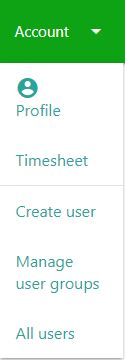
\includegraphics[scale=1]{account_dropdown}
	\caption{Account legördülő menü}
	\label{fig:example-2}
\end{figure}

Az elválasztó vonal alatti almenük: Create user,  Manage user groups, All users csak a rendszergazda jogosultságú felhasználók számára láthatóak. A Logout menüpont értelemszerűen kijelentkezteti a felhasználót.

A főoldal törzsében található 3 opció: Projects - a Projects menüponttal megegyezően a projektek listájára navigál, My open stories - a bejeletnkezett felhasználóhoz rendelt story-k/task-ok/issue-k tekinthetőek meg és a profil adatok, My timesheet - a felhasználó munkaidő könyvelési oldalára kalauzol.

\subsection{Projektek}
\label{projects}

A projektek listájához a Projects menüpont, illetve a főoldalról tudunk eljutni. Az oldalon egyszerre 5 projekt jelenik meg, a többit a \ref{fig:example-3}.ábra alján látható oldal léptetéssel érhetjük el. A projektek létrehozási dátum szerint a legújabbtól haladva a legrégebbi felé jelennek meg. A projekt oldalak esetében a navigációs sávban is megjelenik egy "Create project" neveztű gomb, mellyel egyből a létrehozás oldalra juthatunk.

\begin{figure}[H]
	\centering
	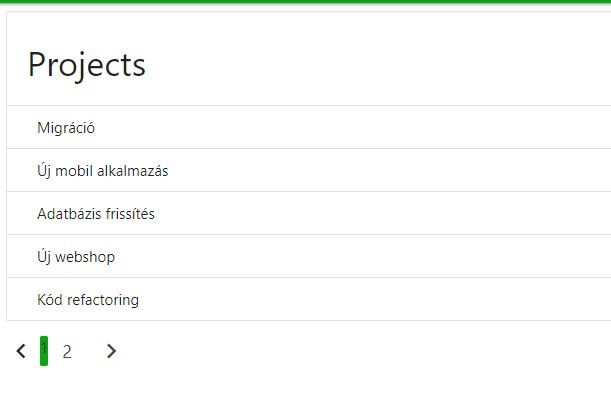
\includegraphics[scale=0.75]{project_list}
	\caption{Projektek listája}
	\label{fig:example-3}
\end{figure}

Az egyes projektekre kattintva eljuthatunk a projekt saját oldalára. Itt megtalálhatjuk az alapvető információkat a projektről, a projektekhez feltöltött dokumentumokat, valamint a projekthez tartozó összes feladat (epic,story,task,issue) felosolását. A jobb alsó sarokban található egy menü, mely az egyes feladat fajták saját oldalain is megtalálhatóak, természetesen részben eltérő menüpontokkal. A projektek esetében ezt tartalmazza a szerkeztés, epic, story, task, issue létrehozását, valamint a projekt szerkeztését, illetve a megfelelő jogosultsággal rendelkezőknek a törlés opciót. (\ref{fig:example-4}. ábra).

\begin{figure}[H]
	\centering
	
\includegraphics[scale=0.75]{edit_menu}
	\caption{almenü, mely különböző opciókat tartalmaz projekt, vagy feladat típustól függően}
	\label{fig:example-4}
\end{figure}

\subsection{Epic, Story, Task, Issue}
\label{stories}

\begin{figure}[H]
	\centering
	\subfigure[Epic]{
		
\includegraphics[scale=1]{epic}}
	\hspace{35pt}
	\subfigure[Story]{
		
\includegraphics[scale=1]{story}}
	\hspace{35pt}
	\subfigure[Task]{
		
\includegraphics[scale=1]{task}}
	\hspace{35pt}
	\subfigure[Issue]{
		
\includegraphics[scale=1]{issue}}
	\caption{Az egyes feladat típusok emblémái}
	\label{fig:example-5}
\end{figure}


\begin{description}
	\item[Epic:] Egy projekten belül levő feladatok gyűjteménye. Mivel projektek több sprinten át élhetnek, ezért rövidebb időszakokban az összefüggő story-k és taskok összefogására érdemes ezt használni. Létrehozni az adott projekt oldalán a korábban említett almenüből lehet (\ref{fig:example-4}. ábra). 
	\item[Story:] Felhasználói feladat. Ha valamilyen jól körülhatárolt fejlesztés van a projekten belül, akkor érdemes ezt használni annak leírására. Létrehozatalkor még nem kötelező hozzárendelni felhasználót, lehet később is a story szerkeztésével. Létrehozni a projekt oldalán levő almenüből (\ref{fig:example-4}. ábra) lehetséges, avagy a navigációs menün megjelenő "Create story" gombra kattintva. Ez olyankor elérhető, amikor egy meglévő story oldalán vagyunk éppen.
	\item[Task:] Szintén felhasználói feladat. A taskot a storyval szemben kisebb feladatok leírására érdemes használni. Például, ha valaki dokumentációt ír, vagy meetingekre jár, vagy csak valami apró fejlesztésről van szó, akkor érdemes azt "taskosítani". Létrehozni a projektek, illetve epicek és storyk oldalán lehetséges (\ref{fig:example-4}. ábra). 
	\item[Issue:] Az issue kicsit eltér a storytól és a tasktól. Az issue valamilyen jellegű probléma leírására használható. Például ha egy elkészült fejlesztésben a teszetelő hibát talál, vagy ha már a leszállított build-ben derül ki valamiféle "bug". Létrehozni a projekt almenüjében lehetséges (\ref{fig:example-4}. ábra).
\end{description}

A story, task és issue hármas státusszal is rendelkezik. Az aktuális státuszt minden olyan oldalon láthatjuk, ahol valamilyen felsorolásban szerepel a 3 közül bármely feladat típus. A státuszt az adott feladat saját oldalán lehet a jobb felső sarokba látható gombbal állítani, melyen mindig az a státusz olvasható, amely az éppen aktuálisat követi.

\begin{figure}[H]
	\centering
	
\includegraphics[scale=1]{storyExample}
	\caption{Példa egy story-ra egy felsorolásban: látható a neve, a projekt kódja, emblémája és aktuális státusza}
	\label{fig:example-6}
\end{figure}

\subsection{Egy példa fejelsztési ciklus}
\label{example_workflow}

Az egyes fogalmak gyorsabb és könnyebb megértése érdekében egy példa fejlesztési folyamaton keresztül szemléltetném a használatukat:

\begin{enumerate}
	\item A scrum master-hez megérkezik a fejlesztési igény (projekt) a klienstől.
	\item Felvesz egy projektet a ScrumHelper-ben. Feltölti hozzá az igényhez kapott dokumentumokat, amelyek segítik majd a tervezők munkáját.
	\item Ezt követően kiosztja az igény megtervezését egy tervezőnek (architect). Ehhez task-ot készít, ahol összeírja a teendőket röviden.
	\item A tervező megírja az igény specifikációját arról, hogyan lehetne ezt az adott rendszerben implementálni (High Level Solution Design).
	\item Utóbbit feltölti a projekt többi dokumentuma közé, majd elkezdi lebontani feladatcsoportokra (epic) és feladatokra (story).
	\item A fejlesztő ezután válogathat a story-k között, melyiket tudja megcsinálni. Amelyiket kiválasztja azt magához rendeli a story szerkeztői oldalán és IN PROGRESS-be rakja a státuszt.
	\item Amint végzett a fejlesztéssel, TESTING státuszba állítja. Egy tesztelő megkeresi (például a Kanban boardon) és magához rendeli.
	\item Ha tesztelés közben hibát talál, akkor felvesz a projekthez egy Issue-t amit az eredeti fejlesztőhöz (vagy aki javítani tudja) rendeli.
	\item Amikor már nincsen probléma a story-val, akkor DONE státuszba rakja.
	\item Egy feladat életciklusának utolsó állomása a CLOSED, amelyre a sprint végén ajánlatos állítani. Ha valami okból újra foglalkozni kell vele, akkor lehetőség van a REOPEN opcióval újra nyitottá tenni.
	\item Egyes Release-k idején, hogy ne legyen túl sok a story, érdemes a rendszergazdáknak egy karbantartó scripttel kiüríteni a már régebben lezárt feladatokat (részletek a \ref{ch:impl}. fejezetben).
\end{enumerate}

\subsection{Kanban tábla}
\label{kanbanboard}

\subsection{Munkaidő könyvelés}
\label{worklog}

